%%%%%%%%%%%%%%%%%%%%%%%%%%%%%%%%%%%%%%%%%
% Beamer Presentation
% LaTeX Template
% Version 1.0 (10/11/12)
%
% This template has been downloaded from:
% http://www.LaTeXTemplates.com
%
% License:
% CC BY-NC-SA 3.0 (http://creativecommons.org/licenses/by-nc-sa/3.0/)
%
%%%%%%%%%%%%%%%%%%%%%%%%%%%%%%%%%%%%%%%%%

%----------------------------------------------------------------------------------------
%	PACKAGES AND THEMES
%----------------------------------------------------------------------------------------
\documentclass{beamer}

\mode<presentation> {

% The Beamer class comes with a number of default slide themes
% which change the colors and layouts of slides. Below this is a list
% of all the themes, uncomment each in turn to see what they look like.

%\usetheme{default}
%\usetheme{AnnArbor}
%\usetheme{Antibes}
%\usetheme{Bergen}
%\usetheme{Berkeley}
%\usetheme{Berlin}
%\usetheme{Boadilla}
%\usetheme{CambridgeUS}
%\usetheme{Copenhagen}
%\usetheme{Darmstadt}
%\usetheme{Dresden}
%\usetheme{Frankfurt}
%\usetheme{Goettingen}
%\usetheme{Hannover}
%\usetheme{Ilmenau}
%\usetheme{JuanLesPins}
%\usetheme{Luebeck}
\usetheme{Madrid}
%\usetheme{Malmoe}
%\usetheme{Marburg}
%\usetheme{Montpellier}
%\usetheme{PaloAlto}
%\usetheme{Pittsburgh}
%\usetheme{Rochester}
%\usetheme{Singapore}
%\usetheme{Szeged}
%\usetheme{Warsaw}

% As well as themes, the Beamer class has a number of color themes
% for any slide theme. Uncomment each of these in turn to see how it
% changes the colors of your current slide theme.

%\usecolortheme{albatross}
%\usecolortheme{beaver}
%\usecolortheme{beetle}
%\usecolortheme{crane}
%\usecolortheme{dolphin}
%\usecolortheme{dove}
%\usecolortheme{fly}
%\usecolortheme{lily}
%\usecolortheme{orchid}
%\usecolortheme{rose}
%\usecolortheme{seagull}
%\usecolortheme{seahorse}
%\usecolortheme{whale}
%\usecolortheme{wolverine}

%\setbeamertemplate{footline} % To remove the footer line in all slides uncomment this line
%\setbeamertemplate{footline}[page number] % To replace the footer line in all slides with a simple slide count uncomment this line

%\setbeamertemplate{navigation symbols}{} % To remove the navigation symbols from the bottom of all slides uncomment this line
}
%----------------------------------------------------------------------------------------
\usepackage{graphicx} % Allows including images
\usepackage{booktabs} % Allows the use of \toprule, \midrule and \bottomrule in tables
\setbeamerfont{caption}{size=\scriptsize}
\usepackage{hyperref}
\usepackage{listings}			%Für C++ Code

%----------------------------------------------------------------------------------------
%	TITLE PAGE
%----------------------------------------------------------------------------------------
\title[]{ROS Basics} % The short title appears at the bottom of every slide, the full title is only on the title page
%----------------------------------------------------------------------------------------
\author{ARRA / AR2A} % Your name
\institute % Your institution as it will appear on the bottom of every slide, may be shorthand to save space
{
\textbf{A}dvancements for \textbf{R}obotics in \textbf{R}escue \textbf{A}pplications
}
\date{\today} % Date, can be changed to a custom date
%----------------------------------------------------------------------------------------
\AtBeginSection{\frame{\sectionpage}}
%----------------------------------------------------------------------------------------
\begin{document}
%----------------------------------------------------------------------------------------
\begin{frame}
\titlepage % Print the title page as the first slide
\end{frame}
%----------------------------------------------------------------------------------------
\begin{frame}
\frametitle{Overview} % Table of contents slide, comment this block out to remove it
\tableofcontents % Throughout your presentation, if you choose to use \section{} and \subsection{} commands, these will automatically be printed on this slide as an overview of your presentation
\end{frame}
%----------------------------------------------------------------------------------------
%	PRESENTATION SLIDES
%----------------------------------------------------------------------------------------
\begin{frame}{ARRA/AR2A}
\begin{large}\textbf{What do we want?}\end{large}
\begin{itemize}
 \item ARRA / AR2A aims to improve the current state of technology of robotics in rescue applications.
\end{itemize}
\begin{large}\textbf{Who are we?}\end{large}
\begin{itemize}
 \item A volunteer non-profit organisation of robotic enthusiasts.
\end{itemize}
\begin{large}\textbf{How can you help?}\end{large}
\begin{itemize}
 \item Check us out at \url{https://github.com/ar2a}
\end{itemize}
 \vspace{1cm}
\begin{large}\textbf{License information}\end{large}
\begin{itemize}
 \item \textbf{CC-BY-SA 4.0} \url{https://creativecommons.org/licenses/by-sa/4.0/}
\end{itemize}
\end{frame}
%----------------------------------------------------------------------------------------
\section{Introduction}
%----------------------------------------------------------------------------------------
\begin{frame}{History}
\begin{itemize}
 \item 2007: Beginnings as project \textbf{switchyard} at the Stanford Artificial Intelligence Laboratory
 \item 2008: Further development by R\&D company Willow Garage  \href{https://www.willowgarage.com/pages/pr2/overview}{\beamergotobutton{PR2}}
 \begin{itemize}
  \item First release: ROS 1.0 (31st December 2012)
 \end{itemize}
 \item 2013: Adoption of the project responsibilty by the \textbf{Open Source Robotics Foundation} (OSRF)
\end{itemize}

\begin{itemize}
 \item \textbf{Versions}: ROS 1.0, Box Turtle, C Turtle, Diamondback, Electric Emys, Fuerte Turtle, Groovy Galapagos, Hydro Medusa, \textbf{Indigo Igloo}, \textbf{Jade Turtle}
 \begin{itemize}
  \item Latest stable version: \textbf{Indigo Igloo}
  \item Latest version: \textbf{Jade Turtle}
 \end{itemize}
\end{itemize}
\end{frame}
%----------------------------------------------------------------------------------------
\begin{frame}{What is ROS?}
\begin{definition}[ROS]
\textit{The Robot Operating System (ROS) is a flexible framework for writing robot software. It is a collection of tools, libraries and conventions that aim to simplify the task of creating complex and robust robot behavior across a wide variety of robotic platforms.}
\end{definition}
\end{frame}
%----------------------------------------------------------------------------------------
\begin{frame}{Why ROS?}
 \begin{itemize}
 \item $>$ \textbf{3000} 3rd party packages in the ROS repositories provide solutions for various, in every robotic system reoccuring problems
 \item Integration with Gazebo, OpenCV, PointCloudLibrary, MoveIt
 \item Extensive documentation and support by a \textbf{vibrant community}
 \begin{itemize}
  \item $>$ \textbf{5700} users at the ROS Q\&{}A-Page (70\%-Answer-Rate)
  \item $>$ \textbf{22000} ROS-Wiki pages
 \end{itemize}
 \item Permissive \textbf{BSD}-Lizenz
 \end{itemize}
 \begin{figure}[H]
  \centering
  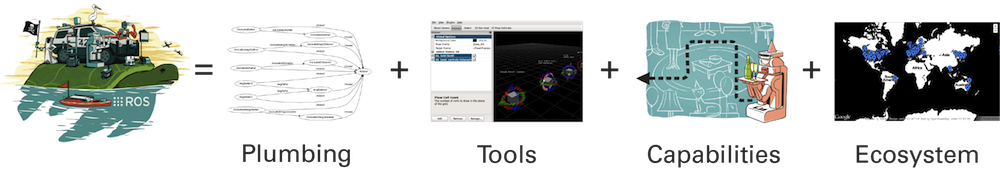
\includegraphics[width=0.85\textwidth]{ros-equation.png}
  \caption{Source: \cite{ROS:2015:Online}}
  \label{fig:ros_equation}
 \end{figure}
\end{frame}
%----------------------------------------------------------------------------------------
\section{Concepts}
%----------------------------------------------------------------------------------------
\begin{frame}{Design Philosophy 1}
 \begin{itemize}
  \item \textbf{Peer-To-Peer}
  \begin{itemize}
   \item Most robotic applications demand a \textbf{huge processing power} 
   \item \textbf{Distributed computing} which performs calculations both on on- and offboard systems required
   \item Interface for data exchange becomes performance bottleneck in systems with a centralised architecture (central server necessary)
  \end{itemize}
 \end{itemize}
 \begin{itemize}
  \item \textbf{Tool based}
  \begin{itemize}
   \item Despite the name \textbf{no operating system but framework} (microkernel approach)
   \item + stability
   \item + expandability
   \item e.g. roscd, roslaunch, rostopic, rosgraph, ...
  \end{itemize}
 \end{itemize}
\end{frame}
%----------------------------------------------------------------------------------------
\begin{frame}{Design Philosophy 2}
 \begin{itemize}
  \item \textbf{Multilingual}
  \begin{itemize}
   \item C++, Python, Octave, Lisp
  \end{itemize}
 \end{itemize}
 \begin{itemize}
  \item \textbf{Thin}
  \begin{itemize}
   \item Encapsulation of algorithms in libraries
   \begin{itemize}
    \item Communication via defined interfaces
    \item Reusability (algorithms are decoupled from hardware)
    \item Easy to test
   \end{itemize}
  \end{itemize}
 \end{itemize}
 \begin{itemize}
  \item \textbf{Open Source}
  \begin{itemize}
   \item BSD license allows for commercial applications without limitations
  \end{itemize}
 \end{itemize}
\end{frame}
%----------------------------------------------------------------------------------------

%----------------------------------------------------------------------------------------
\begin{frame}{Design Philosophy 3}
	
	\begin{definition}[Client Library]
		A Client library implements the core ROS concepts to create nodes, publish and subscribe to topics, write and call services and use the Parameter Server. Such a library can be implemented in any programming language.
	\end{definition}
	
	\begin{itemize}
		\item ROS focus is on robust C++ and Python support. 
		\item ROScpp is designed for high runtime performance
		\item ROSpy favors implementation speed (i.e. developer time) over runtime performance. ROS Master, roslaunch are developed in ROSpy. 
	\end{itemize}
	
\end{frame}
%----------------------------------------------------------------------------------------


%----------------------------------------------------------------------------------------
\subsection{ROS File System}

\begin{frame}{ROS File System}	
	\large{Components}
	
	\begin{itemize}
		\item Packages
		\item Metapackages
		\item Package Manifests
		\item Message types
		\item Service types
		
	\end{itemize}
	
\end{frame}
%----------------------------------------------------------------------------------------

%----------------------------------------------------------------------------------------
\begin{frame}{Packages}	
	
	\begin{definition}[Package]
		\textit{Packages are the most atomic build and release item in ROS. The most granular thing you can build and release is a package. }
	\end{definition}	
	
	A package can contain: 
	\begin{itemize}
		\item ROS runtime processes (nodes)
		\item a ROS-dependent library
		\item datasets 
		\item configuration files
		\item third party piece of software
		\item or anything else that is usefully organized together
	\end{itemize}
	
	It's goal is to provide software in an easy to use (reusable) manner. \\	
		
\end{frame}

%----------------------------------------------------------------------------------------

%----------------------------------------------------------------------------------------
\begin{frame}{Metapackages}	
	
	\begin{definition}[Metapackages]
		A specialized package, which only serves to represent a group of related other packages. 
	\end{definition}
	
	\begin{itemize}
		\item Metapackages do not install files and they do not contain any tests, code, files, or other items usually found in packages. \\
		\item Most commonly metapackages are used as a backwards compatible place holder for converted rosbuild Stacks. 
	\end{itemize}
	
	A Metapackage is like a package with an export tag:
	
	\lstinputlisting[language=XML, ]{Metapackage_Export_Tag.txt}

\end{frame}

%----------------------------------------------------------------------------------------

%----------------------------------------------------------------------------------------
\begin{frame}{Package Manifests}	
	\begin{definition}[Package Manifest]
		The package manifest is an XML file called package.xml. It provides metadata about a package and it must be included with any catkin-compliant package's root folder. 
	\end{definition}
	
	metadata includes: 
	\begin{itemize}
		\item name
		\item version
		\item description
		\item license information
		\item dependencies
		\item other meta information like exported packages
	\end{itemize}
	
\end{frame}

%----------------------------------------------------------------------------------------

%----------------------------------------------------------------------------------------
\begin{frame}{Message types}	
	
	\begin{definition}[Message type]
		A message type is the name of the .msg file and it describes the message (data structure, ...) 
	\end{definition}
		
	\begin{itemize}
		\item Nodes can communicate by publishing Messages to \textbf{topics} or by exchanging a request and response message as part of a ROS \textbf{service} call. \\
		
		\item The .msg file describes the structure of the message (types, arrays, structs, ...). \\
		
		\item The message type is the name of the package + / + msg + / + name of the .msg file. \\
		Example: my\underline{ }package/msg/MyMessageType.msg \\
		
		\item ROS tools automatically generate source code for the message type in several target languages.		
	\end{itemize}

	
\end{frame}

%----------------------------------------------------------------------------------------

%----------------------------------------------------------------------------------------
\begin{frame}{Service types}
	
	\begin{definition}[Service type]
		A service type is the name of the .srv file and it describes the request and response message of the service.
	\end{definition}	
	
	\begin{itemize}
		\item A Service is a pair of messages - request and response. 
		\item Therefore a service type consists of two message types - one for the request and one for the response. 
		\item The service type is the name of the package + / + serv + / + name of the .srv file. \\
		Example: my\underline{ }package/srv/MyServiceType.srv \\
	\end{itemize}
		
\end{frame}

%----------------------------------------------------------------------------------------

%----------------------------------------------------------------------------------------
\subsection{Computation Graph}

%----------------------------------------------------------------------------------------
\begin{frame}{ROS Computation Graph}	
	
	\large{The Computation Graph is the peer-to-peer network of ROS processes that are processing data together.}
	
	\begin{itemize}
		\item Nodes
		\item Messages
		\item Topics
		\item Services
		\item Master
		\item Parameter Server
		\item Bags
	\end{itemize}
	
\end{frame}
%----------------------------------------------------------------------------------------

%----------------------------------------------------------------------------------------
\begin{frame}{Names}
	There are two types of names:
	
	\begin{itemize}
		\item Graph Resource Names
		
			\begin{itemize}
				\item Every computational component (resource = nodes, topics, services, parameters, ...) has an unique name
				\item Each resource is defined within a namespace
				\item A namespace can contain many resources
				\item A resource can create other resources within it's namespace and 
				it can access other resources within or above it's namespace
				\item By default names are resolved relatively
				\item Namespaces provide encapsulation and help to choose the right resource (if there are many with the same name)
			\end{itemize}
		
	\end{itemize}
	
	Every ROS client library supports command-line remapping of names, which means a compiled program can be reconfigured at start-up time to operate in a different Computation Graph topology.
	
\end{frame}
%----------------------------------------------------------------------------------------

%----------------------------------------------------------------------------------------
\begin{frame}{Names}
	\begin{itemize}
		\item Package Resource Names
		
		\begin{itemize}
			\item naming convention to refer to files and datatypes (e.g. Message, Service or Node types) on disk. 
			\item Package Resource Names are similar to file paths, but they are shorter, because ROS assumes their location. \\
			Example: Message descriptions are always stored in the msg subdirectory and have the .msg extension, so std\underline{ }msgs/String is shorthand for path/to/std\underline{ }msgs/msg/String.msg.
			\item Package Resource Names have strict naming rules as they are often used in auto-generated code. 
		\end{itemize}
		
	\end{itemize}
		
\end{frame}
%----------------------------------------------------------------------------------------

\begin{frame}{Nodes}
	\begin{definition}[Node]
		\textit{A node is a process performing calculations.}
	\end{definition}
	
	\begin{itemize}
		\item Typical applications consist of multiple nodes
		\item Naming results from graphical representation of all running processes and the communication between those processes as \textbf{directed graph} (Tool: \textit{rqt\_graph})
		\item Identification of a process by a \textbf{graph ressource name} (''Nodename'')
		\begin{figure}[H]
			\centering
			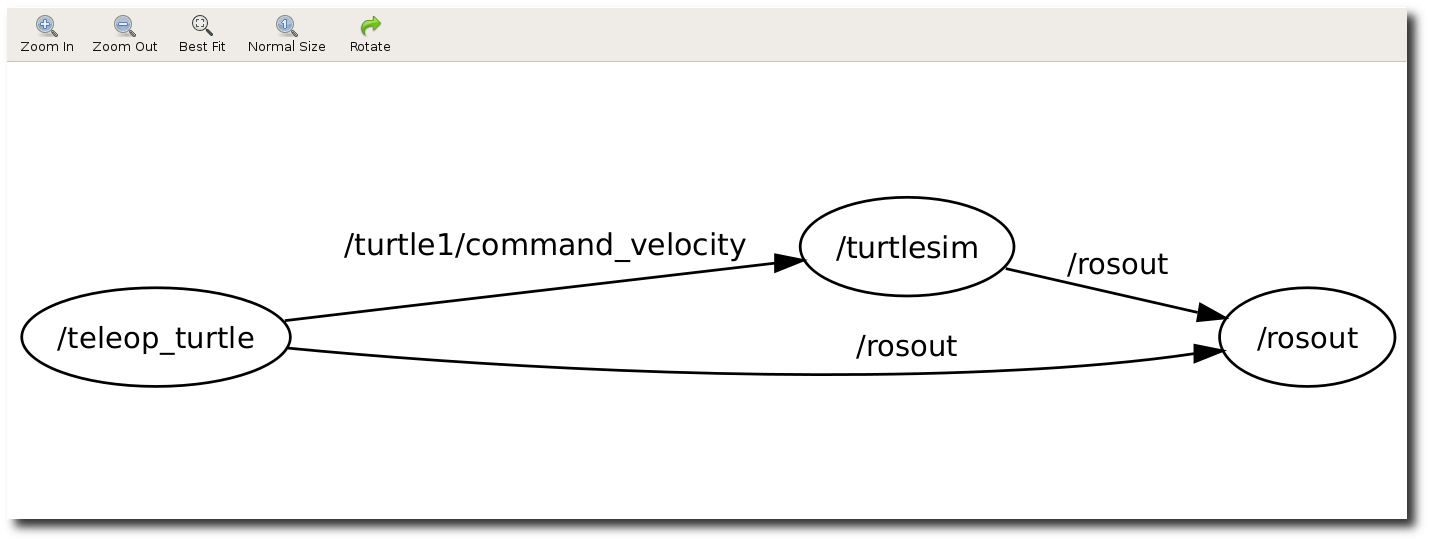
\includegraphics[width=0.6\textwidth]{rxgraph-turtle-key.png}
			\caption{Source: \cite{ROS:2015:Online}}
			\label{fig:ros_graph}
		\end{figure}
	\end{itemize}
\end{frame}
%----------------------------------------------------------------------------------------

\begin{frame}{Nodes}
		
	Advantages of nodes:
	
	\begin{itemize}
		\item More fault tolerance as crashes are isolated to individual nodes \\
		
		\item Code complexity is reduced
		\item Implementation details are well hidden as the nodes expose a minimal API to the rest of the graph 
	\end{itemize}
\end{frame}
%----------------------------------------------------------------------------------------

%----------------------------------------------------------------------------------------

\begin{frame}{Messages}
	\begin{definition}[Messages]
		\textit{Messages are a means of communication. A message is a simple data structure comprising typed fields. }
	\end{definition}
	
	Topics and services use messages, as already describe at the Message Types slide.
	
\end{frame}
%----------------------------------------------------------------------------------------


\begin{frame}{Topic}
	\begin{definition}[Topic]
		\textit{A topic is a unique name which allows nodes to locate their communication partner for the transmission and reception of data.}
	\end{definition}
	\begin{itemize}
		\item Creation and consumption of data is \textbf{decoupled} (Producer/Consumer-Pattern)
		\begin{itemize}
			\item Source's (\textbf{publish}) data to a topic
			\item Sink's (\textbf{subscribe}) data from a topic
		\end{itemize}
		\begin{figure}[H]
			\centering
			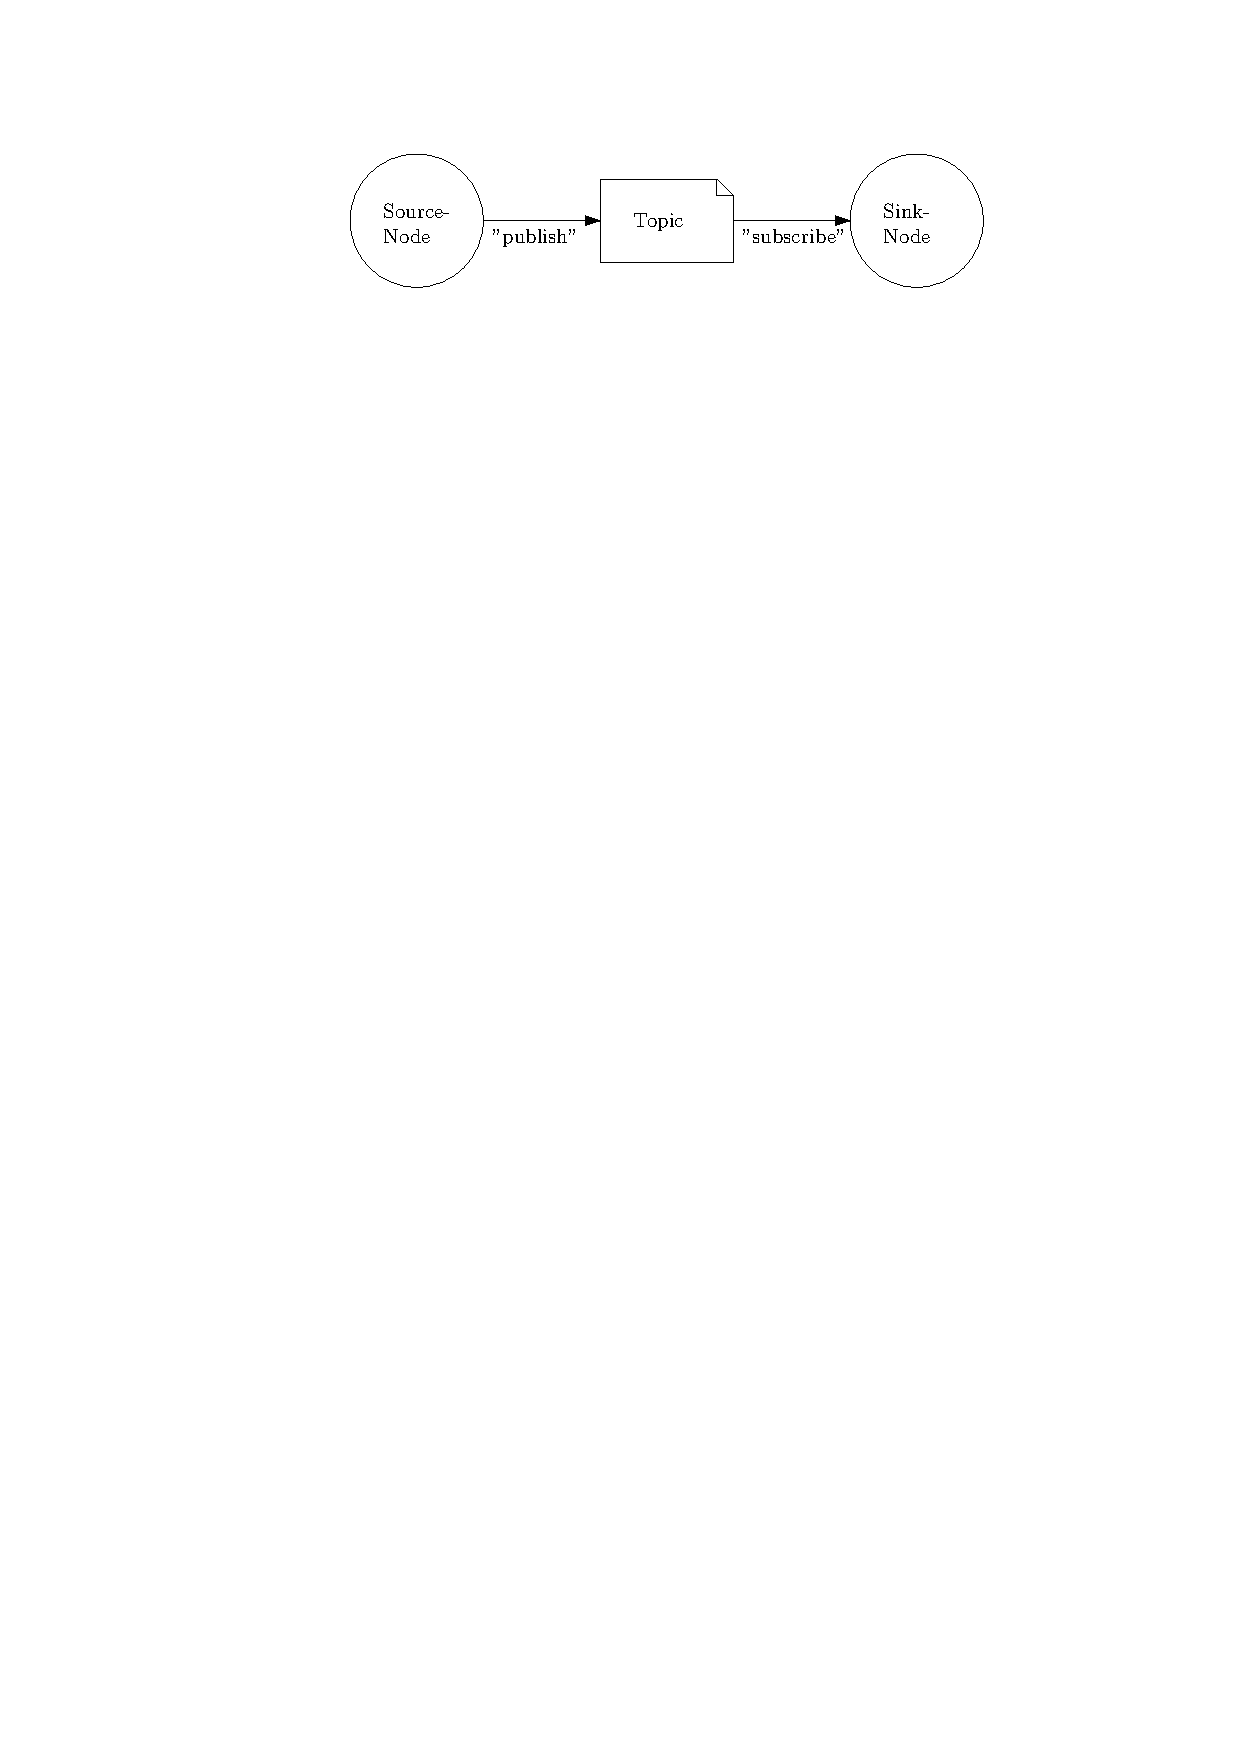
\includegraphics[width=0.6\textwidth]{ros-topic.pdf}
			\label{fig:ros_topic}
		\end{figure}
		\item \textbf{Unidirectional} communication
		\item \textit{Point to Point} and \textit{Point to Multipoint}
	\end{itemize}
\end{frame}
%----------------------------------------------------------------------------------------
\begin{frame}{Service}
	\begin{definition}[Service]
		\textit{Services allow for bidirectional communication between two nodes in form of request/response couples.}
	\end{definition}
	\begin{itemize}
		\item \textbf{Request} $\rightarrow$ $Node_1$ requests a service from $Node_2$ (e.g. addition)
		\item \textbf{Response} $\rightarrow$ $Node_2$ executes service and returns result to $Node_2$
		\item 
		\begin{figure}[H]
			\centering
			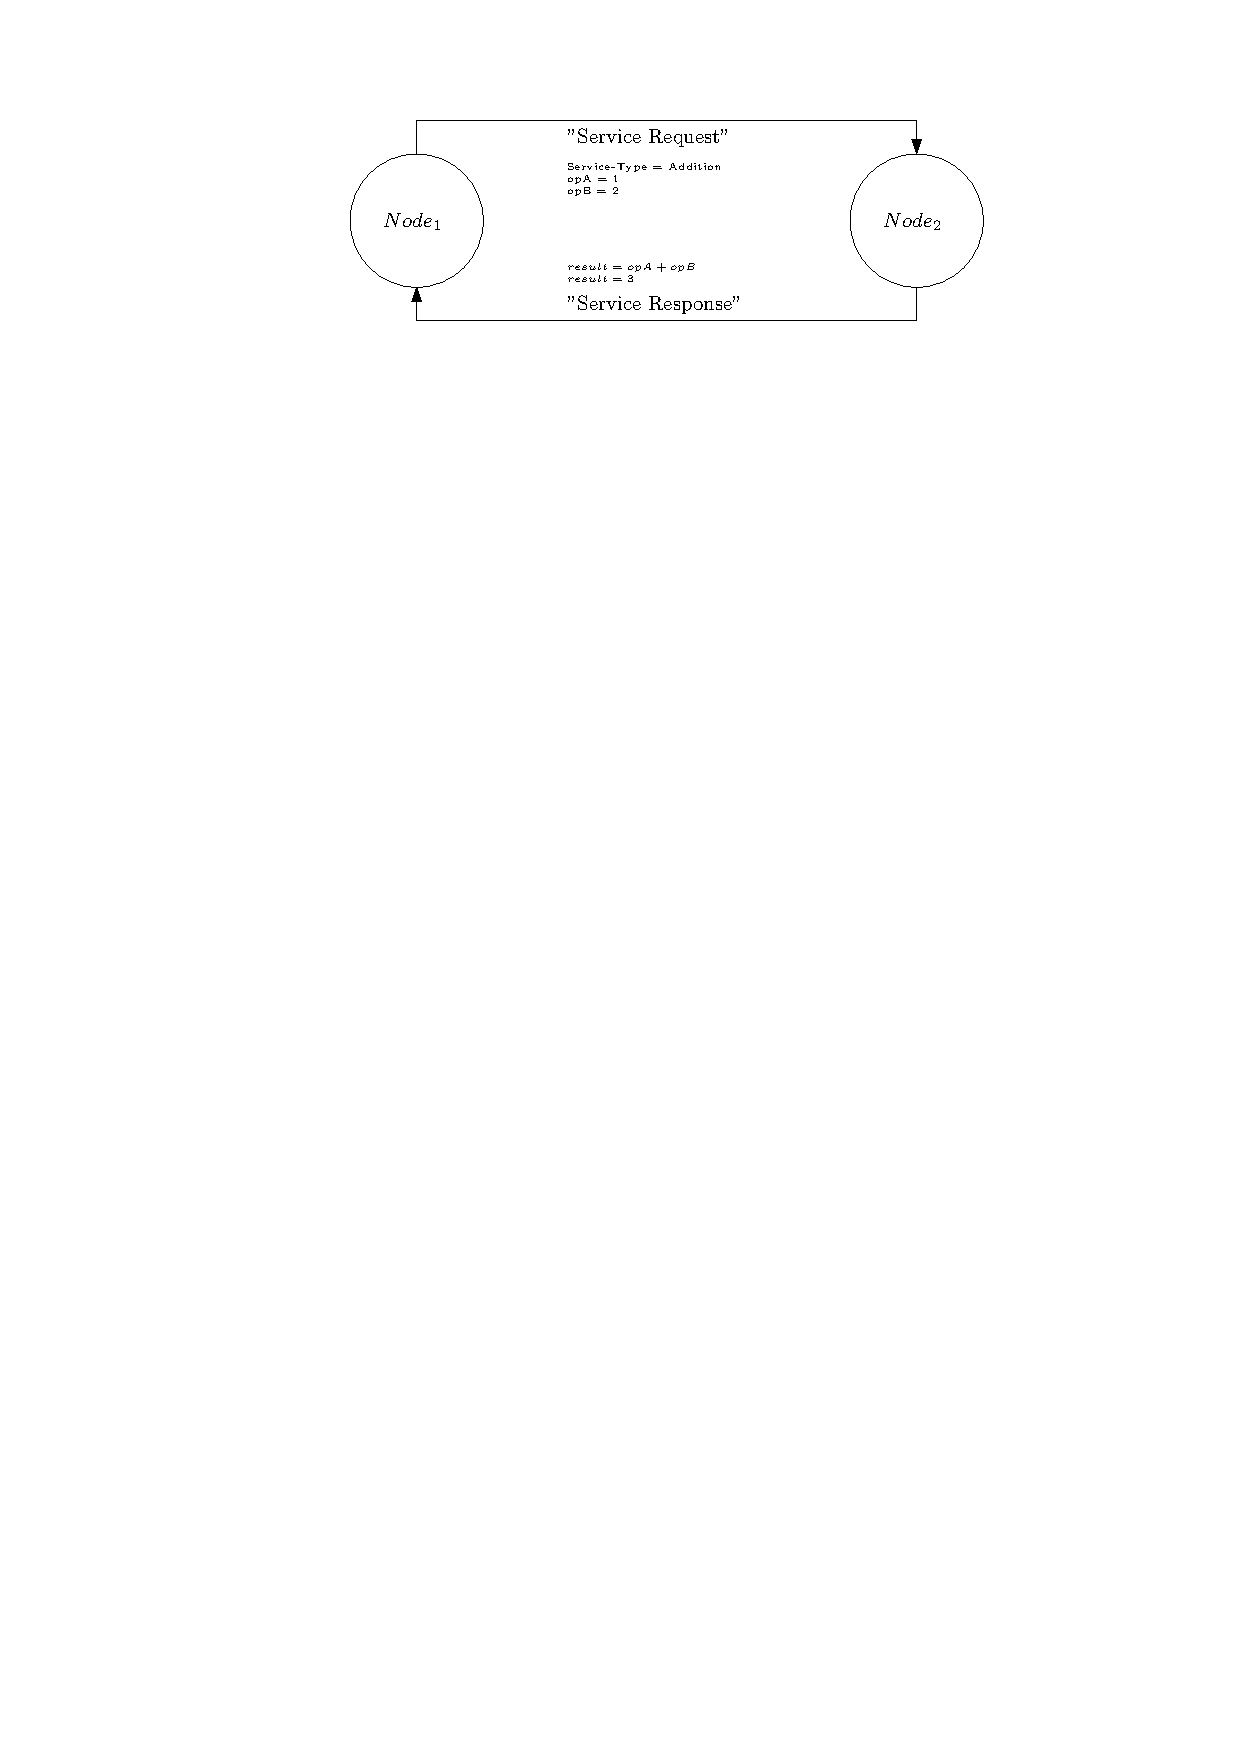
\includegraphics[width=0.6\textwidth]{ros-service.pdf}
			\label{fig:ros_service}
		\end{figure}
		\item Concrete implementation as a \textbf{remote procedure call}
		\item \textbf{Bidirectionale} (\textit{Point to Point}) communication
	\end{itemize}
\end{frame}
%----------------------------------------------------------------------------------------


%----------------------------------------------------------------------------------------
\begin{frame}{Master}
	\begin{definition}[Master]
		\textit{The ROS Master provides name registration and lookup to the rest of the Computation Graph.}
	\end{definition}
	
	\begin{itemize}
		\item acts as a nameservice 
		\item stores topics and service registration information for ROS nodes
		\item nodes ask the master for information about other nodes, then the nodes connect to other nodes directly (TCPROS: TCP/IP sockets) -  the Master only provides lookup information
		\item the master makes callbacks to these nodes when the registration information changes -  nodes can create dynamic connections as new nodes are run
		
	\end{itemize}
	Without the Master nodes would not be able to find each other, exchange messages, or invoke services.
	
\end{frame}
%----------------------------------------------------------------------------------------

%----------------------------------------------------------------------------------------
\begin{frame}{Master Example}
	
	There are two Nodes. A Camera node and an Image\underline{ }viewer node. The Camera notifies the master that it wants to publish images on the topic "images":
	 
		  \begin{figure}[H]
		  	\centering
		  	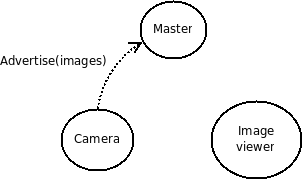
\includegraphics[scale=0.7]{ROS_master_example_english_1.png}
		  	\caption{Master Example 1}
		  	\label{fig:ros_master_example_1}
		  \end{figure}
	
	
\end{frame}
%----------------------------------------------------------------------------------------

%----------------------------------------------------------------------------------------
\begin{frame}{Master Example}
	
	Camera publishes images to the "images" topic, but nobody is subscribing to that topic yet so no data is actually sent. \\ 
	Then the Image\underline{ }viewer subscribes to the topic "images" to see if there are some images there: 
	
	\begin{figure}[H]
		\centering
		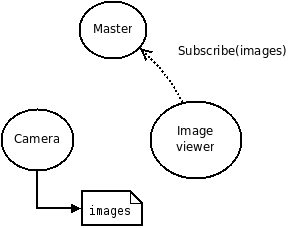
\includegraphics[scale=0.6]{ROS_master_example_english_2.png}
		\caption{Master Example 2}
		\label{fig:ros_master_example_2}
	\end{figure}
	
	
\end{frame}
%----------------------------------------------------------------------------------------

%----------------------------------------------------------------------------------------
\begin{frame}{Master Example}
	
	Now that the topic "images" has both a publisher and a subscriber, the master node notifies Camera and Image\underline{ }viewer about each others existence so that they can start transferring images to one another: 
	
	\begin{figure}[H]
		\centering
		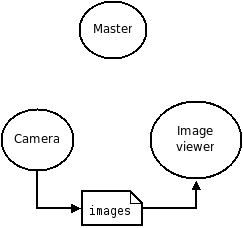
\includegraphics[scale=0.65]{ROS_master_example_english_3.png}
		\caption{Master Example 3}
		\label{fig:ros_master_example_3}
	\end{figure}
	
	
\end{frame}
%----------------------------------------------------------------------------------------

%----------------------------------------------------------------------------------------
\begin{frame}{Parameter Server}
	\begin{definition}[Parameter Server]
		\textit{The Parameter Server allows data to be stored by key in a central location. It is a shared, multi-variate dictionary that is accessible via network APIs.}
	\end{definition}
	
	\begin{itemize}
		\item The Parameter Server is part of the Master.
		\item It's globally viewable so tools can easily inspect the configuration state of the system and modify it if necessary. 
	\end{itemize}
	
	\textbf{Example:} Define the following parameters: \\
	/gains/P = 10.0 \\
	/gains/I = 1.0 \\
	/gains/D = 0.1 \\
	
	Read separately: /gains/P $\rightarrow$ returns  10.0 \\
	or read the whole dictionary: /gains $\rightarrow$ \{ 'P': 10.0, 'I': 1.0, 'D' : 0.1 \}
	
\end{frame}
%----------------------------------------------------------------------------------------


%----------------------------------------------------------------------------------------
\begin{frame}{ROS Core}
	\begin{definition}[ROS Core]
		roscore is a collection of nodes and programs that are pre-requisites of a ROS-based system (they have to run in order for ROS nodes to communicate).
	\end{definition}
	
	\begin{itemize}
		\item use "roscore" command to launch it ("roslaunch" command starts roscore automatically too)
		\item the roscore includes the master, parameter server and a rosout logging node  
	\end{itemize}	
	
\end{frame}
%----------------------------------------------------------------------------------------


%----------------------------------------------------------------------------------------
\begin{frame}{Bags}
	\begin{definition}[Bag]
		A bag is a file format in ROS for storing ROS message data. It's a primary mechanism in ROS for data logging and has a variety of offline uses.  
	\end{definition}
	\begin{itemize}
		\item Bags are created by a tool like rosbag, which subscribes to one or more ROS topics, and stores the serialized message data in a file as it is received. 
		\item The bag files can be played back in ROS to the same topics they were recorded from, or even remapped to new topics. 
	\end{itemize}
	Bags are a format for saving and playing back ROS message data. Bags are an important mechanism for storing data, such as sensor data, that can be difficult to collect but is necessary for developing and testing algorithms.	
	
\end{frame}
%----------------------------------------------------------------------------------------


\section{Useful Means}

%----------------------------------------------------------------------------------------
\begin{frame}{Useful Means}

	\begin{itemize}
		\item \textbf{tf package:} A framework for calculating the positions of multiple coordinate frames over time. \\
		  
		\item \textbf{actionlib package:} The actionlib defines a common, topic-based interface for preemptible tasks in ROS.
		
		\item \textbf{common\underline{ }msgs Stack:} 
			\begin{itemize}
				\item actionlib\underline{ }msgs: messages for representing actions
				\item diagnostic\underline{ }msgs: messages for sending diagnostic data
				\item geometry\underline{ }msgs: messages for representing common geometric primitives
				\item nav\underline{ }msgs: messages for navigation
				\item sensor\underline{ }msgs: messages for representing sensor data
			\end{itemize}
				
	\end{itemize}

\end{frame}
%----------------------------------------------------------------------------------------

%----------------------------------------------------------------------------------------
\begin{frame}{Useful Means}
	
	\begin{itemize}
		\item \textbf{pluginlib:} It provides a library for dynamically loading libraries in C++ code. 
		
		\item \textbf{filters package:} It provides a C++ library for processing data using a sequence of filters.
		
		\item \textbf{urdf package:} It defines an XML format for representing a robot model and provides a C++ parser. 
		
		\item \textbf{rqt:} rqt is a Qt-based framework for GUI development for ROS. 
		
		\item \textbf{ROS Cheat Sheet}
		
	\end{itemize}
	
\end{frame}
%----------------------------------------------------------------------------------------

%----------------------------------------------------------------------------------------
\begin{frame}{dynamic\underline{ }reconfigure}
	\begin{definition}[dynamic\underline{ }reconfigure]
		dynamic\underline{ }reconfigure is a package which allows you to reconfigure a subset of a node's parameters at any time without having to restart the node. 
	\end{definition}
	
	\begin{itemize}

		\item Client programs (e.g. GUIs) can query a node for it's set of reconfigureable parameters (name, type, range of the param)
		
		\item the API is still under development $\rightarrow$ significant changes expected
		
		\item a reconfigure\underline{ }gui tool is provided in the rqt library
		
		\item the dynparam command-line tool is stable $\rightarrow$ \\
		rosrun dynamic\underline{ }reconfigure dynparam COMMAND
		
		\item the python API is stable, a C++ API is not yet implemented, but you can use the system command as a workaround. 
		
		
	\end{itemize}
	
	
	
\end{frame}
%----------------------------------------------------------------------------------------


\begin{frame}[allowframebreaks]{References}
\scriptsize{\bibliographystyle{ieeetr}}
\bibliography{references} %bibtex file name without .bib extension
\end{frame}
%----------------------------------------------------------------------------------------
\begin{frame}
\Huge{\centerline{The End}}
\end{frame}
%----------------------------------------------------------------------------------------
\end{document} 
%----------------------------------------------------------------------------------------